%%*************************************************************************
%% Legal Notice:
%% This code is offered as-is without any warranty either expressed or
%% implied; without even the implied warranty of MERCHANTABILITY or
%% FITNESS FOR A PARTICULAR PURPOSE! 
%% User assumes all risk.
%% In no event shall the IEEE or any contributor to this code be liable for
%% any damages or losses, including, but not limited to, incidental,
%% consequential, or any other damages, resulting from the use or misuse
%% of any information contained here.
%%
%% All comments are the opinions of their respective authors and are not
%% necessarily endorsed by the IEEE.
%%
%% This work is distributed under the LaTeX Project Public License (LPPL)
%% ( http://www.latex-project.org/ ) version 1.3, and may be freely used,
%% distributed and modified. A copy of the LPPL, version 1.3, is included
%% in the base LaTeX documentation of all distributions of LaTeX released
%% 2003/12/01 or later.
%% Retain all contribution notices and credits.
%% ** Modified files should be clearly indicated as such, including  **
%% ** renaming them and changing author support contact information. **
%%*************************************************************************

% *** Authors should verify (and, if needed, correct) their LaTeX system  ***
% *** with the testflow diagnostic prior to trusting their LaTeX platform ***
% *** with production work. The IEEE's font choices and paper sizes can   ***
% *** trigger bugs that do not appear when using other class files.       ***                          ***
% The testflow support page is at:
% http://www.michaelshell.org/tex/testflow/


\documentclass[conference]{IEEEtran}
% Some Computer Society conferences also require the compsoc mode option,
% but others use the standard conference format.
%
% If IEEEtran.cls has not been installed into the LaTeX system files,
% manually specify the path to it like:
% \documentclass[conference]{../sty/IEEEtran}


% Some very useful LaTeX packages include:
% (uncomment the ones you want to load)


% *** MISC UTILITY PACKAGES ***
%
%\usepackage{ifpdf}
% Heiko Oberdiek's ifpdf.sty is very useful if you need conditional
% compilation based on whether the output is pdf or dvi.
% usage:
% \ifpdf
%   % pdf code
% \else
%   % dvi code
% \fi
% The latest version of ifpdf.sty can be obtained from:
% http://www.ctan.org/pkg/ifpdf
% Also, note that IEEEtran.cls V1.7 and later provides a builtin
% \ifCLASSINFOpdf conditional that works the same way.
% When switching from latex to pdflatex and vice-versa, the compiler may
% have to be run twice to clear warning/error messages.


% *** CITATION PACKAGES ***
%
%\usepackage{cite}
% cite.sty was written by Donald Arseneau
% V1.6 and later of IEEEtran pre-defines the format of the cite.sty package
% \cite{} output to follow that of the IEEE. Loading the cite package will
% result in citation numbers being automatically sorted and properly
% "compressed/ranged". e.g., [1], [9], [2], [7], [5], [6] without using
% cite.sty will become [1], [2], [5]--[7], [9] using cite.sty. cite.sty's
% \cite will automatically add leading space, if needed. Use cite.sty's
% noadjust option (cite.sty V3.8 and later) if you want to turn this off
% such as if a citation ever needs to be enclosed in parenthesis.
% cite.sty is already installed on most LaTeX systems. Be sure and use
% version 5.0 (2009-03-20) and later if using hyperref.sty.
% The latest version can be obtained at:
% http://www.ctan.org/pkg/cite
% The documentation is contained in the cite.sty file itself.


% *** GRAPHICS RELATED PACKAGES ***
%
\ifCLASSINFOpdf
  % \usepackage[pdftex]{graphicx}
  % declare the path(s) where your graphic files are
  % \graphicspath{{../pdf/}{../jpeg/}}
  % and their extensions so you won't have to specify these with
  % every instance of \includegraphics
  % \DeclareGraphicsExtensions{.pdf,.jpeg,.png}
\else
  % or other class option (dvipsone, dvipdf, if not using dvips). graphicx
  % will default to the driver specified in the system graphics.cfg if no
  % driver is specified.
  % \usepackage[dvips]{graphicx}
  % declare the path(s) where your graphic files are
  % \graphicspath{{../eps/}}
  % and their extensions so you won't have to specify these with
  % every instance of \includegraphics
  % \DeclareGraphicsExtensions{.eps}
\fi
% graphicx was written by David Carlisle and Sebastian Rahtz. It is
% required if you want graphics, photos, etc. graphicx.sty is already
% installed on most LaTeX systems. The latest version and documentation
% can be obtained at: 
% http://www.ctan.org/pkg/graphicx
% Another good source of documentation is "Using Imported Graphics in
% LaTeX2e" by Keith Reckdahl which can be found at:
% http://www.ctan.org/pkg/epslatex
%
% latex, and pdflatex in dvi mode, support graphics in encapsulated
% postscript (.eps) format. pdflatex in pdf mode supports graphics
% in .pdf, .jpeg, .png and .mps (metapost) formats. Users should ensure
% that all non-photo figures use a vector format (.eps, .pdf, .mps) and
% not a bitmapped formats (.jpeg, .png). The IEEE frowns on bitmapped formats
% which can result in "jaggedy"/blurry rendering of lines and letters as
% well as large increases in file sizes.
%
% You can find documentation about the pdfTeX application at:
% http://www.tug.org/applications/pdftex

\usepackage{tikz}
\usetikzlibrary{trees}


% *** MATH PACKAGES ***
%
\usepackage{amsmath}
% A popular package from the American Mathematical Society that provides
% many useful and powerful commands for dealing with mathematics.
%
% Note that the amsmath package sets \interdisplaylinepenalty to 10000
% thus preventing page breaks from occurring within multiline equations. Use:
%\interdisplaylinepenalty=2500
% after loading amsmath to restore such page breaks as IEEEtran.cls normally
% does. amsmath.sty is already installed on most LaTeX systems. The latest
% version and documentation can be obtained at:
% http://www.ctan.org/pkg/amsmath


% *** SPECIALIZED LIST PACKAGES ***
%
%\usepackage{algorithmic}
% algorithmic.sty was written by Peter Williams and Rogerio Brito.
% This package provides an algorithmic environment fo describing algorithms.
% You can use the algorithmic environment in-text or within a figure
% environment to provide for a floating algorithm. Do NOT use the algorithm
% floating environment provided by algorithm.sty (by the same authors) or
% algorithm2e.sty (by Christophe Fiorio) as the IEEE does not use dedicated
% algorithm float types and packages that provide these will not provide
% correct IEEE style captions. The latest version and documentation of
% algorithmic.sty can be obtained at:
% http://www.ctan.org/pkg/algorithms
% Also of interest may be the (relatively newer and more customizable)
% algorithmicx.sty package by Szasz Janos:
% http://www.ctan.org/pkg/algorithmicx


% *** ALIGNMENT PACKAGES ***
%
%\usepackage{array}
% Frank Mittelbach's and David Carlisle's array.sty patches and improves
% the standard LaTeX2e array and tabular environments to provide better
% appearance and additional user controls. As the default LaTeX2e table
% generation code is lacking to the point of almost being broken with
% respect to the quality of the end results, all users are strongly
% advised to use an enhanced (at the very least that provided by array.sty)
% set of table tools. array.sty is already installed on most systems. The
% latest version and documentation can be obtained at:
% http://www.ctan.org/pkg/array

% IEEEtran contains the IEEEeqnarray family of commands that can be used to
% generate multiline equations as well as matrices, tables, etc., of high
% quality.


% *** SUBFIGURE PACKAGES ***
%\ifCLASSOPTIONcompsoc
%  \usepackage[caption=false,font=normalsize,labelfont=sf,textfont=sf]{subfig}
%\else
%  \usepackage[caption=false,font=footnotesize]{subfig}
%\fi
% subfig.sty, written by Steven Douglas Cochran, is the modern replacement
% for subfigure.sty, the latter of which is no longer maintained and is
% incompatible with some LaTeX packages including fixltx2e. However,
% subfig.sty requires and automatically loads Axel Sommerfeldt's caption.sty
% which will override IEEEtran.cls' handling of captions and this will result
% in non-IEEE style figure/table captions. To prevent this problem, be sure
% and invoke subfig.sty's "caption=false" package option (available since
% subfig.sty version 1.3, 2005/06/28) as this is will preserve IEEEtran.cls
% handling of captions.
% Note that the Computer Society format requires a larger sans serif font
% than the serif footnote size font used in traditional IEEE formatting
% and thus the need to invoke different subfig.sty package options depending
% on whether compsoc mode has been enabled.
%
% The latest version and documentation of subfig.sty can be obtained at:
% http://www.ctan.org/pkg/subfig


% *** FLOAT PACKAGES ***
%
%\usepackage{fixltx2e}
% fixltx2e, the successor to the earlier fix2col.sty, was written by
% Frank Mittelbach and David Carlisle. This package corrects a few problems
% in the LaTeX2e kernel, the most notable of which is that in current
% LaTeX2e releases, the ordering of single and double column floats is not
% guaranteed to be preserved. Thus, an unpatched LaTeX2e can allow a
% single column figure to be placed prior to an earlier double column
% figure.
% Be aware that LaTeX2e kernels dated 2015 and later have fixltx2e.sty's
% corrections already built into the system in which case a warning will
% be issued if an attempt is made to load fixltx2e.sty as it is no longer
% needed.
% The latest version and documentation can be found at:
% http://www.ctan.org/pkg/fixltx2e

%\usepackage{stfloats}
% stfloats.sty was written by Sigitas Tolusis. This package gives LaTeX2e
% the ability to do double column floats at the bottom of the page as well
% as the top. (e.g., "\begin{figure*}[!b]" is not normally possible in
% LaTeX2e). It also provides a command:
%\fnbelowfloat
% to enable the placement of footnotes below bottom floats (the standard
% LaTeX2e kernel puts them above bottom floats). This is an invasive package
% which rewrites many portions of the LaTeX2e float routines. It may not work
% with other packages that modify the LaTeX2e float routines. The latest
% version and documentation can be obtained at:
% http://www.ctan.org/pkg/stfloats
% Do not use the stfloats baselinefloat ability as the IEEE does not allow
% \baselineskip to stretch. Authors submitting work to the IEEE should note
% that the IEEE rarely uses double column equations and that authors should try
% to avoid such use. Do not be tempted to use the cuted.sty or midfloat.sty
% packages (also by Sigitas Tolusis) as the IEEE does not format its papers in
% such ways.
% Do not attempt to use stfloats with fixltx2e as they are incompatible.
% Instead, use Morten Hogholm'a dblfloatfix which combines the features
% of both fixltx2e and stfloats:
%
% \usepackage{dblfloatfix}
% The latest version can be found at:
% http://www.ctan.org/pkg/dblfloatfix


% *** PDF, URL AND HYPERLINK PACKAGES ***
%
%\usepackage{url}
% url.sty was written by Donald Arseneau. It provides better support for
% handling and breaking URLs. url.sty is already installed on most LaTeX
% systems. The latest version and documentation can be obtained at:
% http://www.ctan.org/pkg/url
% Basically, \url{my_url_here}.


% *** Do not adjust lengths that control margins, column widths, etc. ***
% *** Do not use packages that alter fonts (such as pslatex).         ***
% There should be no need to do such things with IEEEtran.cls V1.6 and later.
% (Unless specifically asked to do so by the journal or conference you plan
% to submit to, of course. )


% correct bad hyphenation here
% \hyphenation{op-tical net-works semi-conduc-tor}


\begin{document}
%
% paper title
% Titles are generally capitalized except for words such as a, an, and, as,
% at, but, by, for, in, nor, of, on, or, the, to and up, which are usually
% not capitalized unless they are the first or last word of the title.
% Linebreaks \\ can be used within to get better formatting as desired.
% Do not put math or special symbols in the title.
\title{Modularization as a Leverage to Facilitate Trustworthiness of Neural Networks}


% author names and affiliations
% use a multiple column layout for up to three different
% affiliations
%\author{
%    \IEEEauthorblockN{Lukas Friedrichsen}
%    \IEEEauthorblockA{Bochum University of Applied Sciences\\
%    D 42579 Heiligenhaus, Germany\\
%    Email: lukas.friedrichsen@hs-bochum.de}
%    \and
%    \IEEEauthorblockN{Jörg Frochte}
%    \IEEEauthorblockA{Bochum University of Applied Sciences\\
%    D 42579 Heiligenhaus, Germany\\
%    Email: joerg.frochte@hs-bochum.de}
%}
\author{
    \IEEEauthorblockN{someone 1}
    \IEEEauthorblockA{a university\\
    somewhere in the world\\
    Email: someone1@xyz.com}
    \and
    \IEEEauthorblockN{someone 2}
    \IEEEauthorblockA{a university\\
    somewhere in the world\\
    Email: someone2@xyz.com}
}


% conference papers do not typically use \thanks and this command
% is locked out in conference mode. If really needed, such as for
% the acknowledgment of grants, issue a \IEEEoverridecommandlockouts
% after \documentclass

% for over three affiliations, or if they all won't fit within the width
% of the page, use this alternative format:
% 
%\author{\IEEEauthorblockN{Michael Shell\IEEEauthorrefmark{1},
%Homer Simpson\IEEEauthorrefmark{2},
%James Kirk\IEEEauthorrefmark{3}, 
%Montgomery Scott\IEEEauthorrefmark{3} and
%Eldon Tyrell\IEEEauthorrefmark{4}}
%\IEEEauthorblockA{\IEEEauthorrefmark{1}School of Electrical and Computer Engineering\\
%Georgia Institute of Technology,
%Atlanta, Georgia 30332--0250\\ Email: see http://www.michaelshell.org/contact.html}
%\IEEEauthorblockA{\IEEEauthorrefmark{2}Twentieth Century Fox, Springfield, USA\\
%Email: homer@thesimpsons.com}
%\IEEEauthorblockA{\IEEEauthorrefmark{3}Starfleet Academy, San Francisco, California 96678-2391\\
%Telephone: (800) 555--1212, Fax: (888) 555--1212}
%\IEEEauthorblockA{\IEEEauthorrefmark{4}Tyrell Inc., 123 Replicant Street, Los Angeles, California 90210--4321}}


% use for special paper notices
%\IEEEspecialpapernotice{(Invited Paper)}


% make the title area
\maketitle


% As a general rule, do not put math, special symbols or citations
% in the abstract
\begin{abstract}

The progress in Deep Learning (DL) in recent years has led to many new, previously inaccessible fields of activity now being opened up. At the same time, however, the requirements in aspects such as scalability, transparency and trust have increased as well. To address this, we propose modularization as a technique to reduce hardware requirements for training and inference of models and to facilitate knowledge transfer, error traceability and interpretability / transparency of predictions. In this work, we focus on the latter two aspects and examine the central question whether the approach can be utilized to incentivize neural networks to learn conceptual relationships between the different categories and hence increase the trustworthiness of predictions. We restrict our considerations to the most common forms of modularization and assess the approach on a qualitative basis. Using an augmented version of the CIFAR100 dataset, we experimentally investigate the impact of modularization on the predictive conceptual proximity of CNNs. The results indicate that by means of modularization a good compromise between trustworthiness and performance can be achieved.

\end{abstract}

% no keywords


% For peer review papers, you can put extra information on the cover
% page as needed:
% \ifCLASSOPTIONpeerreview
% \begin{center} \bfseries EDICS Category: 3-BBND \end{center}
% \fi
%
% For peerreview papers, this IEEEtran command inserts a page break and
% creates the second title. It will be ignored for other modes.
% \IEEEpeerreviewmaketitle


\section{Introduction%
         \label{sec:introduction}}

The progress in image recognition in the last two decades has been nothing short of astonishing, not least due to the success of CNNs (\cite{Alom2018-yo}). However, as a consequence of the ongoing endeavor to solve evermore complex tasks, many modern models can't be economically feasibly trained anymore without computing capacities that necessitate access to datacenters or cloud platforms. Being neither a completely novel nor in itself negative development, it does effect a drastic reduction in practical applicability and facilitates an increasing oligopolization of the Deep Learning industry as well as research in favor of those with access to more resources and / or data. This is further catalyzed by the inherent limitation of DL regarding the impossibility to refactor once learnt knowledge and the requirement to retrain the whole model each time a shift in the data base occurs.

Moreover, the decision-making process of conventional neural networks is difficult to comprehend due to their inherent nature. The latter is, however, becoming more and more important as such systems are increasingly employed in safety-critical applications such as autonomous driving or for predictions with high economic implications. It is undisputed that Trustworthy AI is a prerequisite for the public acceptance of DL.

To address these shortcomings, we propose the modularization of neural networks in abstraction of the well-known "divide and conquer" principle from computer science. This work is part of a wider study on this topic, focusing on the aspect of interpretability and model trustworthiness in particular.

Specifically, we argue that by explicitly inferring the structure of the label space into the model architecture, the network is incentivized to learn conceptual relationships between the different categories. In other words, predictions by a modularized network are on average conceptually closer to the ground truth than those of conventional neural networks.

As a positive ancillary effect, decomposition simplifies the interpretability of the model's decision making process since humans equally tend to decompose complex problems into simpler sub-problems; hence, forecasts based on several iterative sub-decisions are easier to comprehend than monolithic predictions without intermediate results.

While the presented concepts are theoretically transferable to arbitrary models, in this work we limit our focus to Directed Acyclic Graphs, in particular CNNs as a subcategory of neural networks.

In summary, this paper has the following contributions: We first discuss advantages and disadvantages of the presented approach. Subsequently, a general theoretical foundation regarding the modularization of neural networks is given. Specifically, different ways to decompose a network are analyzed, the impact of modularization on convergence and performance properties of a model are discussed and the concept of modularization error is introduced.

In a dedicated section we debate different aspects of trustworthy AI and how to measure them. In this regard, we extend the concept of semantic distance established by \cite{Fergus2010-or} to be able to effectively compare different models on this basis.

We do then present two experiments in which we compare a modularized network and a comparable conventional CNN on an augmented version of the CIFAR100 dataset to assess how the presented technique affects the model's behavior with regard to its predictive conceptual proximity. Our findings suggest that, at the expense of a slight decrease of absolute performance, modularization does indeed incentivize the model to learn conceptual relationships, resulting in more trustworthy predictions. The work is concluded by a summarizing discussion of the results.

\begin{figure}
    \centering
    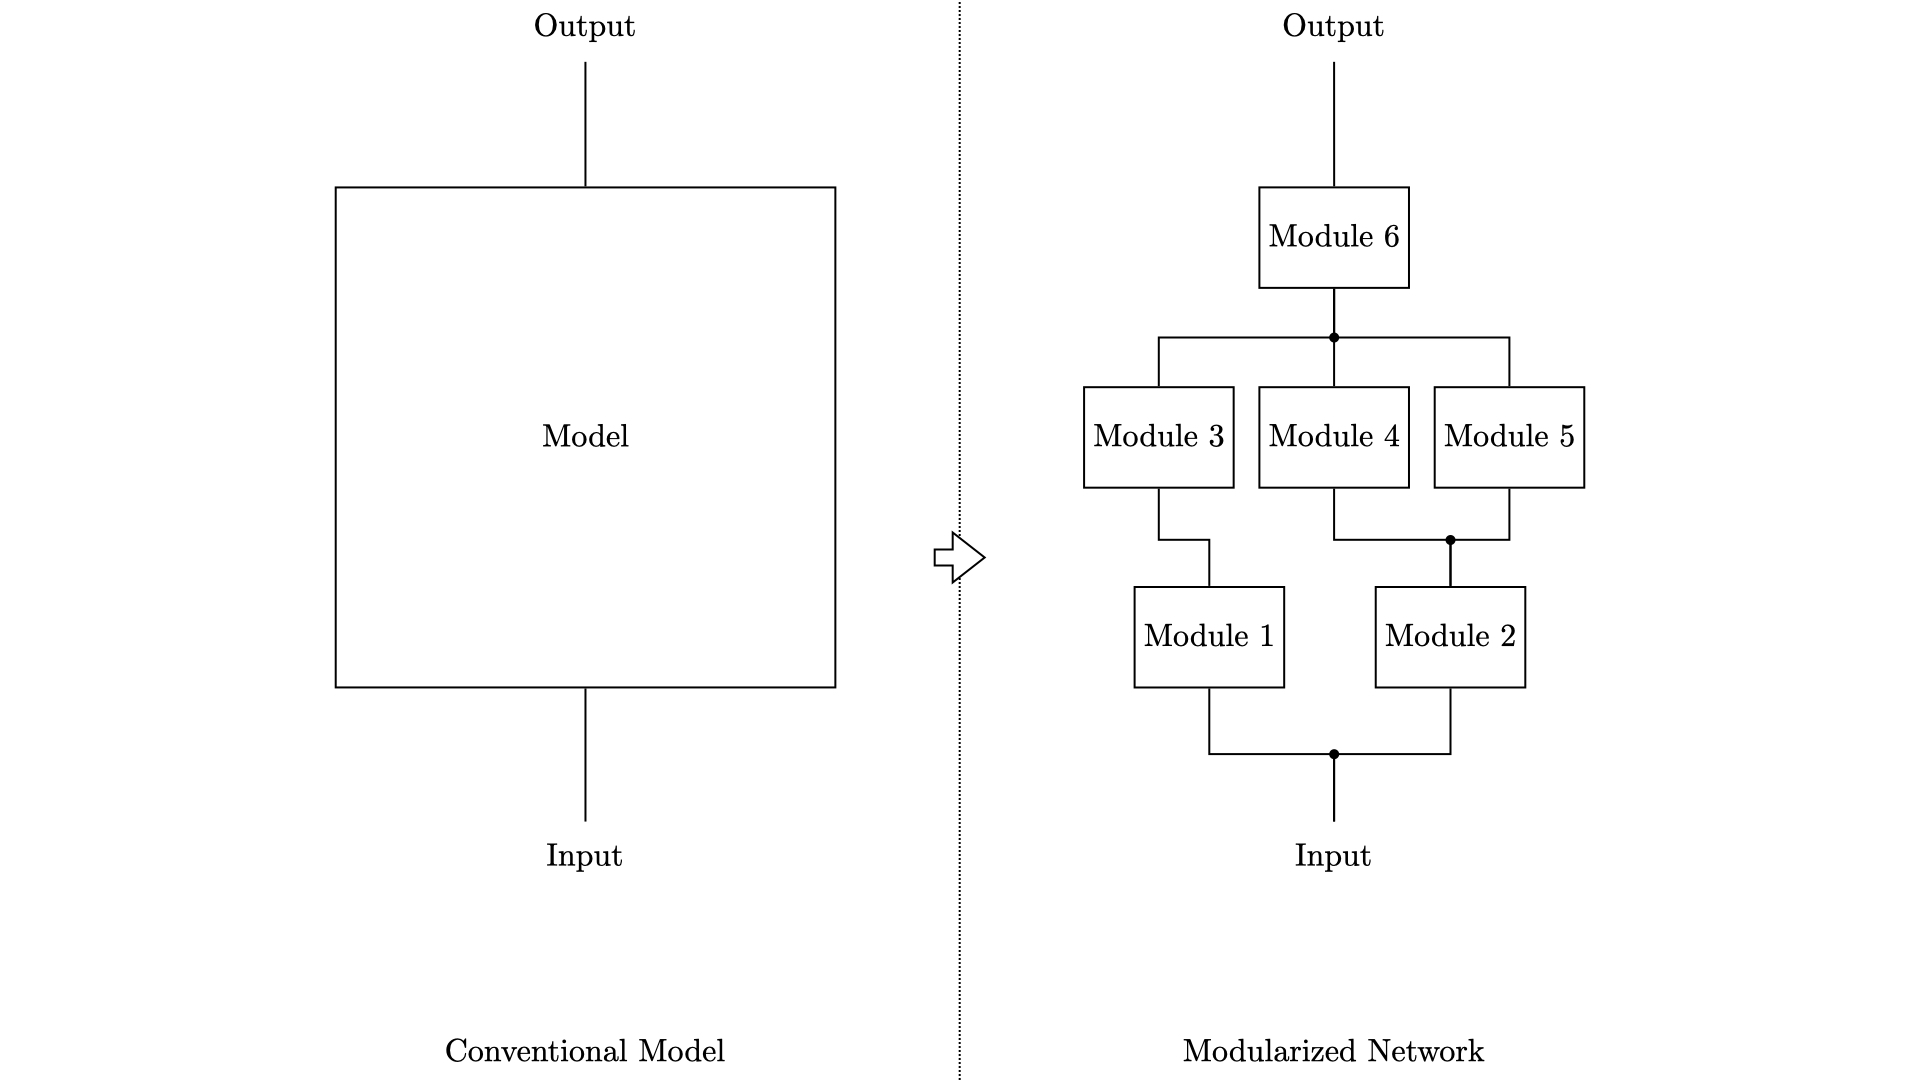
\includegraphics[width=\linewidth, trim=325 0 325 0, clip]{graphics/basic_concept.jpeg}
    \caption{The basic idea: By explicitly inferring structural information into the model, modularization facilitates behavioral comprehensibility of neural networks and incentivizes conceptual proximity of predictions.}
    \label{fig:introduction_basic_concept}
\end{figure}

\section{Related Work%
         \label{sec:related_work}}

The idea of composing a single model from multiple submodules is not a novel one; Initial approaches to combine multiple learners dating back to the late 80s originated from the domain of competitive learning, mainly born as an approach to overcome the limitations of computational resources that served as the primary bottleneck in machine learning (ML) at that time.

Early works such as \cite{Jacobs1991-fo} and \cite{Jacobs1991-rz} develop "divide and conquer" strategies to have different networks compete for subspaces of the domain, facilitated by gating networks that learn to dynamically switch between the submodules depending on the input. Adopting a similar philosophy, \cite{Jordan1994-gn} derive a stochastic framework for the "divide and conquer" approach; i.\,e.\ the model is trained using a variant of the EM (Expectation Maximization) algorithm to learn a mixture of probabilities from which the final result is then drawn. The authors argue that such an approach not only decreases hardware requirements but also increases learning speed and interpretability, reduces spatial and temporal crosstalk and leads to better generalization.

Early general studies on consensus theory in non-competitive modular systems can be found in \cite{Benediktsson1992-bl} and \cite{Xu1992-hp}. These works, however, focus on the combination of different independently trained learners to reduce uncertainty and error rates when compared to the individual composing submodules. An overview of the fields in which modularization is employed for task-independent performance boosting today can e.\,g.\ be found in \cite{Alpaydin2019-nh}.

Concerning task-specific developments leveraging modularization, especially in image recognition, composed approaches have become increasingly popular in research since the establishment of publicly accessible, large-scale datasets with multiple label hierarchy levels such as CIFAR100 or ImageNet in the last decade.

E.\,g.\ \cite{Yan2015-go} propose a network composed of multiple template models. They employ unsupervised learning techniques to identify natural clusters of alike classes and train one building block model for each meta-concept found this way. Thereby the authors aim to maximize the decision boundaries between categories and optimize the usage of modeling capacity per individual module. Their work suggests the validity of the approach and devises different techniques to further reduce hardware requirements for composed models.

A very recent publication originating from a different point of view by \cite{Roy2020-rv} employs tree-like, dynamically growing structures of CNNs to combat what the authors denote as "catastrophic forgetting" in image recognition, i.\,e.\ networks forgetting learned patterns when they are retrained on new data. Furthermore, the authors argue that a modular structure facilitates expendability and adaptability of DL models for situations where new data becomes steadily available or a constant distributional shift takes place as is the case in many real-world scenarios.

Most recent findings in the form of \cite{Filan2020-nx} furthermore suggest that neural networks in general tend to naturally form modular clusters when being trained using modern regularization techniques such as Pruning or Dropout and might thus be inherently accessible to modularization.

\section{Advantages of a Modular Model Structure%
         \label{sec:advantages}}

In theory, modular design introduces several desirable characteristics with regard to practical applicability of neural networks. In the following, a brief overview of the different benefits of modularization is given.

Firstly, a network composed from multiple submodules has the advantage of providing several breakpoints throughout the decision making process. It de facto breaks up the black box that is a monolithic model and provides insights in how the final prediction is formed, thus facilitating comprehensibility of the model's behavior. We hypothesize that part of the reason for the above is that this kind of incremental reasoning is closer to the human decision making process, similar to how we also naturally tend to break down complex problems in smaller, simpler ones. Hence, forecasts based on several iterative sub-decisions are easier to comprehend than monolithic predictions without intermediate results.

Secondly, being able to trace the decision making process throughout the network through the interim results of the different submodules equally facilitates traceability of errors and identification of error sources in general. I.\,e.\ by tracing the flow of information through the composed network, it is possible to perform post-mortem analysis of error causality and location. While the former provides an understanding of the nature of the error, the latter indicates where exactly adjustments have to be made to fix this deficit. Both are highly desirable characteristics in practice, especially for applications with safety implications that necessitate deterministic traceability of failures. Moreover, a modular structure allows for the incorporation of deterministic modules such as error detection mechanisms or fallback routines in addition to conventional network elements (in the sense of "hybrid models") which can contribute to achieving predictable model behavior and ensuring trustworthiness.

Other benefits of modularization include enhanced retrainability and modifiability / extensibility of models, simplified refactoring of once-learnt knowledge -- either through transfer learning or the outright reuse of entire submodules in different composed networks -- and facilitated accessibility of ML in hardware constrained environments by reduction of the minimal necessary computing power for training and inference.

Concluding, modularization offers various benefits in comparison to conventional monolithic networks, in particular flexibility / modifiability and trustworthiness / interpretability, the latter being the focus of this work.

\section{Composition of Meta-Networks from Multiple Submodules%
         \label{sec:compnet}}

\subsection{Decomposable Dimensions of Neural Networks%
            \label{sec:compnet_dimensions}}
            
\begin{figure*}
    \centering
    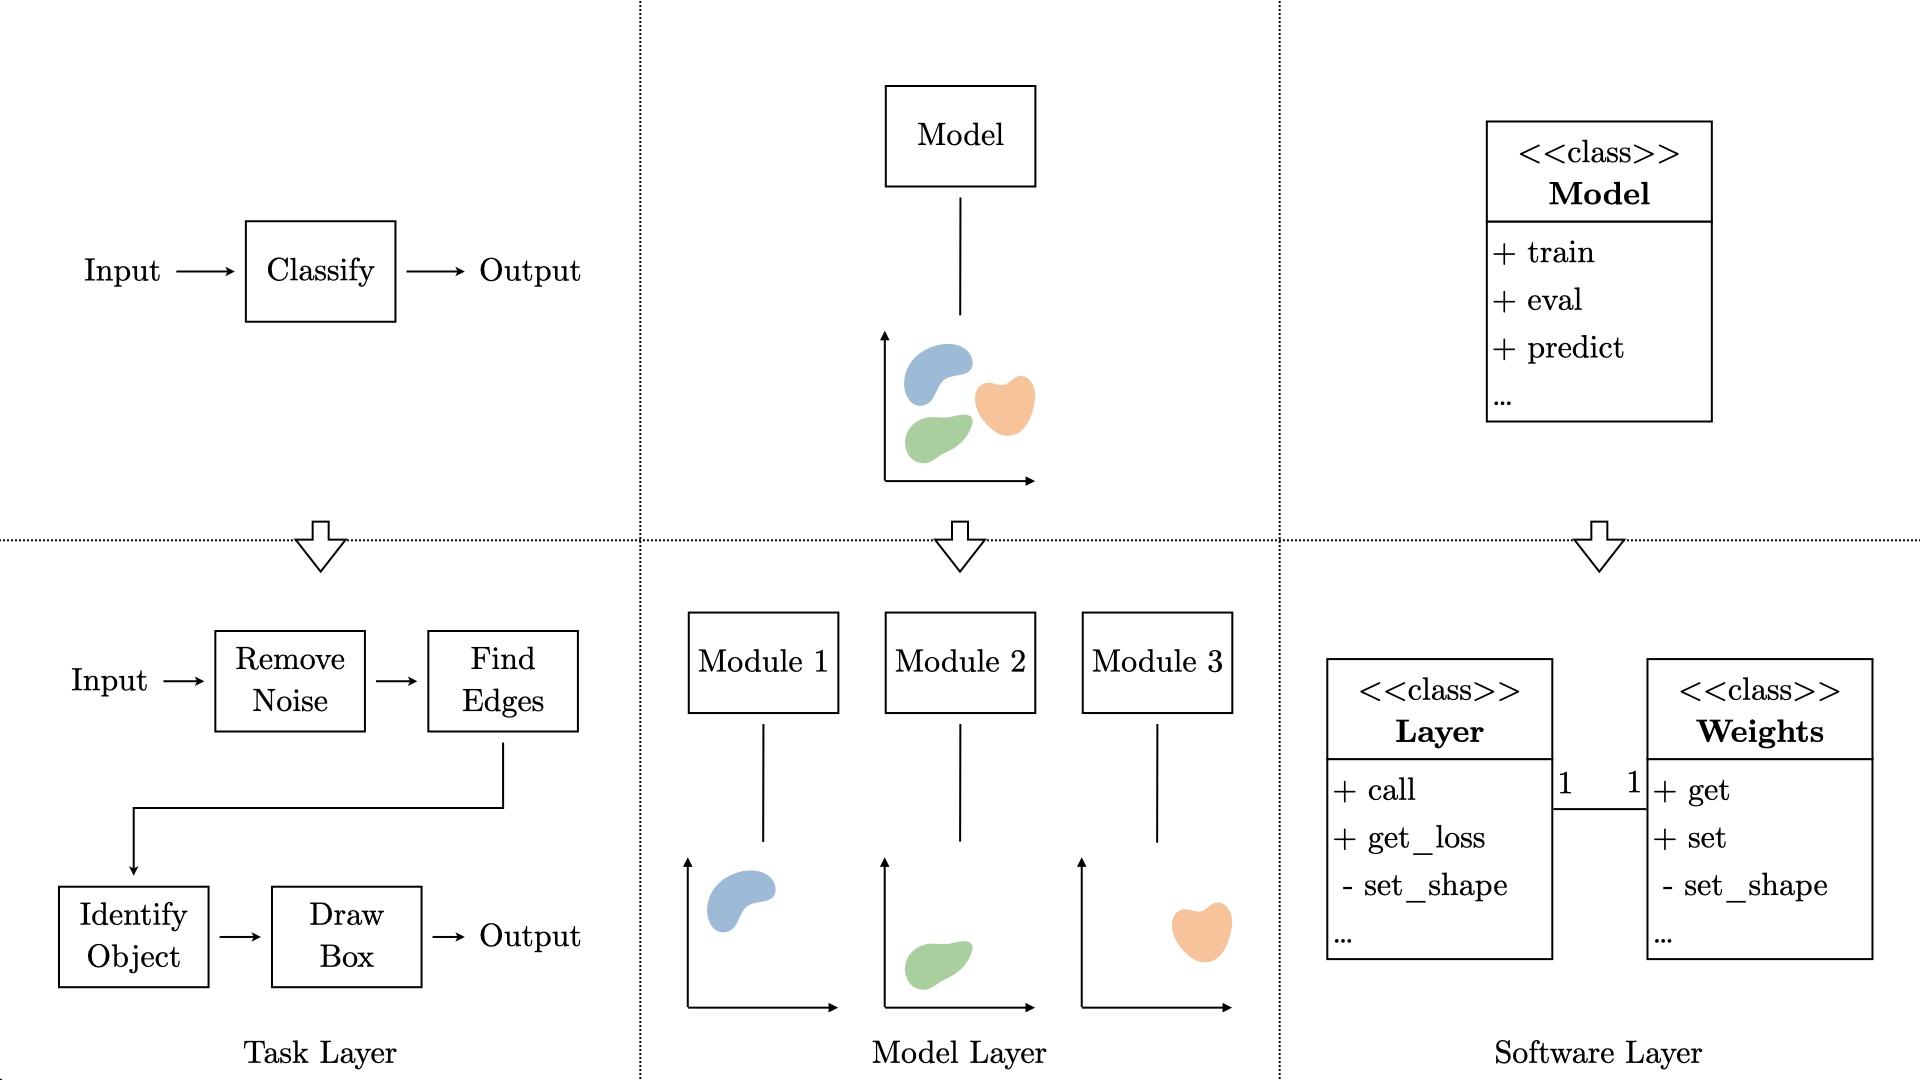
\includegraphics[width=0.85\textwidth, trim=0 -25 0 -25, clip]{graphics/dimension.jpeg}
    \caption{Modularization can be applied to any of the three domains constituting a specific model instantiation.}
    \label{fig:compnet_dimensions}
\end{figure*}

To resolve the ambiguity of the term modularization in the context of ML, we begin by identifying the different dimensions of neural networks to which the technique is applicable.

Consider an arbitrary ML model. While seeming like a single, cohesive system on the surface, it is in reality constituted from multiple different dimensions characterizing the concrete instantiation of the model:

\vspace{\baselineskip}
\begin{itemize}
    \item \textbf{Task:} A task is an algorithmic description of a particular process relating a specific input to a specific output that can be expressed by means of mathematical or natural language statements. Every particular model instantiation is coupled to a specific, existence-giving task. It is the purpose of the model to learn the transformation defined by the latter.
    \item \textbf{Model:} Model in this case refers to the functional depiction of the pivotal task as well as all related sub-tasks. This includes aspects such as the concrete type and architecture of the employed model, preprocessing routines, training and testing procedures, etc.
    \item \textbf{Implementation:} Ultimately, every model is a piece of software. It can be interpreted as a projection of the functional model to the computational level. While not inferring any information on its own, the implementation very well affects the overall system in aspects such as (computational) performance, modifiability, etc.
\end{itemize}
\vspace{\baselineskip}
            
Modularization as a technique is applicable to any of the aforementioned dimensions and yields different effects depending on the context (cf.\ figure \ref{fig:compnet_dimensions}).

For instance, the modeled task can be separated into several sub-tasks based on its inherent nature, that is, if it can be interpreted as a meta-task composed of multiple smaller tasks. The model layer directly reflects such decompositions on the task layer. However, within these constraints, modularization can occur independent of the considered process as well, e.\,g.\ motivated by the inherent structure of the underlying data base.

Both modularization on the task as well as on the model layer infer information augmenting the topology of the search space into the model. We denote this as auxiliary information in contrast to primary information, i.\,e.\ knowledge contained in the relation between domain and codomain. Specifically, modularization enhances the structure of the search space by introducing additional constraints, effectively dividing it into several sparsely connected subspaces, each of which is of lower complexity than the composed space. The amount of auxiliary information inferred by a particular decomposition is proportional to the amount as well as the strictness (i.\,e.\ holonomic or non-holonomic) of the introduced constraints. Consequently, the existing modeling capacity can be utilized more efficiently as the amount of information the model has to learn explicitly is reduced.

The increased specificity of the model, however, results in a reduction of the generalizability at the same time as described by the "No Free Lunch" theorem by \cite{Wolpert1997-fu}. Hence modularization is always case specific and can hardly be transferred between tasks. I.\,e.\, while the submodules can easily be reused in other applications, the individual decomposition has to be conceived anew for each new model.

The software layer on the other hand does not infer any information into the system. It can thus be designed in an arbitrarily modularized way as long as the projection of the functional model is retained. As mentioned before, this may still impact aspects such as modifiability or computational performance.

\subsection{Types of Modularization%
            \label{sec:compnet_types}}

There are two fundamental ways to decompose a system into submodules, horizontal and vertical decomposition. Note that with "system", we denote any structure or process that transforms an arbitrary input into an equally arbitrary output here. Both types of modularization act on the transformation from domain to codomain and are not mutually exclusive, i.\,e.\ they are freely combinable.

\textbf{Horizontal Modularization:} Horizontal modularization describes the process of decomposing an arbitrary process in a suitable way to approximate a parental process through multiple parallel (optimally independent) sub-processes. From a mathematical point of view, the decomposition can be understood as an optimization problem where a transformation from a certain domain to a codomain is to be separated in a way that the informational loss in comparison to the original transformation is to be minimized. For an optimal decomposition, the resulting modules are capable of modelling the primary information in its entirety; the auxiliary information inherently increases due to the additional holonomic constraints inferred by the separation into individual submodules. In consequence, the resulting meta-network learns faster but not necessarily better. Three forms of horizontal modularization are possible:

\vspace{\baselineskip}
\begin{itemize}
    \item Decomposition in the domain with unchanged codomain and reconstruction of the original transformation via aggregation of the results of the different submodules
    \item Decomposition in the codomain with unchanged domain and reconstruction of the original transformation via merging / superimposing of the subspaces of the different submodules
    \item Arbitrary combinations of the former two
\end{itemize}
\vspace{\baselineskip}

\textbf{Vertical Modularization:} Vertical modularization, also known as Layering, describes the process of modulating the information channel along which the primary information in the domain is mapped to the codomain by decomposing a process into different sub-processes, also called Layers, along the axis of transformation. The amount of primary information in the system is restricted by the maximum amount the informationally most limited layer can store. In other words, if e.\,g.\ any of the intermediate layers in a modular system possesses a single Boolean as sole output, it is impossible for outputs of subsequent layers (and thus the overall model) to be of higher complexity without additional input. Note, however, that the amount of primary information a layer can contain is composed of the cardinality as well as the interrelations of the states within the layer. Thus a pure dimensionality reduction from one layer to the next does not necessarily imply loss of information. Similar to horizontal modularization, vertical modularization increases the auxiliary information and hence the specificity of the system.

Popular applications leveraging vertical modularization e.\,g.\ include contemporary Natural Language Processing architectures that chain neural networks and autoencoders.
            
\subsection{Convergence and Performance Properties%
            \label{sec:compnet_convergence_performance}}

An interesting and certainly legitimate question in regard to composed networks is whether, just because convergence was guaranteed for a given model before modularization, this property is retained after decomposition as well. Alas, answering this is beyond the scope of this paper. Luckily, however, in practice it is usually the opposite directionality that is of much more relevance and which can be established easily by inductive reasoning:

\vspace{\baselineskip}
\newtheorem{theorem}{Theorem}
\begin{theorem}
    Consider a network composed from multiple submodules. If all individual modules of this network converge, the overall model converges as well.
\end{theorem}
\vspace{\baselineskip}

Intuitively, the meta-search space of the overall model is the superposition of the individual modules' sub-search spaces. Similarly, the optimum in the composite space is formed by superimposing the optima of the subspaces. Obviously, as long as all submodules converge against their respective optima, the overall model equally converges. If all subspaces are disjoint, the resulting meta-optimum is a point; otherwise it consists of a higher dimensional region.

Note, however, that the optimum found this way is not necessarily the global optimum of the meta-space. The problem of finding a decomposition that guarantees the latter is strongly related to the question posed at the beginning of this section and as such equally beyond the scope of this work.

Conversely, convergence within the individual submodules can be understood as convergence in the meta-space along the dimensions of the respective subspace against the projection of the meta-optimum to this subspace. This is comparable to freezing all DOFs of the meta-space except for the ones of a specific submodule and solely performing optimization, e.\,g.\ via SGD (Stochastic Gradient Descent), on the remainder. Albeit the fineness of the descent consequently decreases, the convergence properties remain unaffected.

As an additional observation, the maximum improvement of performance a composed network can achieve over a comparative monolithic model is limited to the amount of information immanent to the modularization. If the modularization does not add any auxiliary information to the model, the original search space is retained and the global optimum remains the same in consequence as well. More specific decompositions infer more prior knowledge and hence the higher the theoretically possible performance gain; the model becomes more susceptible to modularization error at the same time, however (cf.\ section \ref{sec:compnet_error}).
            
\subsection{Modularization Error%
            \label{sec:compnet_error}}

A major challenge of modularization is finding a suitable decomposition that projects the prior knowledge concerning the structure of task or data base to the model without at the same time causing the loss of pivotal primary information e.\,g.\ due to oversimplification, etc. Noteworthily, the information is not really lost; the decomposition simply causes the network to lose the capability to model certain interrelations in this case due to the inferred constraints. Hence decomposition on the task and model layer can have adverse effects on the performance of the model if it decomposes the overall search space in a way that the theoretically optimal solution is located outside of the subspaces. We denote this as a suboptimal decomposition and the resulting deviation between theoretic optimum and closest reachable configuration within the composed search space as modularization error.

Furthermore, even if an optimal decomposition can be found, modularization may also affect the topology of the search space in a way that the inherent characteristics of optima finding algorithms -- most commonly SGD -- are affected negatively (e.\,g.\ by resulting in subspaces that are almost completely sparse). This may additionally impact efficiency and performance of the model.

Consequently, finding a suitable decomposition is a sensitive issue and should always be performed on a per-model basis for the performance loss due to modularization errors not to outweigh the practical advantages of the approach.

\section{Measuring Model Trustworthiness%
         \label{sec:semantic_distance}}

While we consider it to be self-evident that, through explicit structural definition and the availability of interim results, modularization simplifies interpretability and facilitates error traceability, the implications of the approach on model trustworthiness necessitate further investigation.

First and foremost, the question arises as to what constitutes trustworthiness in relation to neural networks. According to the "Ethics guidelines for trustworthy AI" by the European Commission (\cite{Robotics_and_Artificial_Intelligence_Unit_A_12019-of}), trustworthy AI must be lawful, ethical and robust. While the first lawfulness and ethicality are arguably abstract concepts, robustness is again subdivided into different technical aspects such as transparency and reliability. In this paper, we focus on the latter; in particular, we argue that a pivotal factor of reliability that is facilitated by modularization is the predictive conceptual proximity of a model, i.\,e.\ how close faulty predictions are on average to the ground truth on a conceptual level.

To elaborate this point, consider e.\,g.\ the obstacle detection system of an autonomous vehicle. In this case it is of less importance for such a system to be able to accurately tell apart \textit{men} and \textit{woman} than it is for it reliably distinguish between \textit{humans} and e.\,g.\ \textit{road signs}. This we denote as predictive conceptual proximity.

To measure this property, we employ semantic distance as defined by \cite{Fergus2010-or} as

\begin{equation*}
    S_{i, j} = \frac{\operatorname{intersect}(\operatorname{path}(i), \operatorname{path}(j))}{\max(\operatorname{length}(\operatorname{path}(i)), \operatorname{length}(\operatorname{path}(j)))}
\end{equation*}

where $\operatorname{path}(i)$ is the path from the root node to the $i$-th node in a hierarchical label structure as we use it in our experiments. I.\,e.\, the higher the semantic distance, the closer the two concepts are related. Measured over a set of $n$ samples, it is hence possible to obtain an average semantic distance for a whole model as

\begin{equation*}
    \bar{S} = \frac{1}{n} \cdot \sum^n{S_{predicted, ground\_truth}}
\end{equation*}

This metric is, however, directly dependent on the absolute accuracy of the respective network. This makes it a poor choice when comparing two different models with differing performance levels. Consider e.\,g.\ two networks, one with a top-1 accuracy of 70\% and an average semantic distance of 0.7 and one with a top-1 accuracy of 50\% and a semantic distance of 0.65. Solely asking which of both has better learned categorical interrelations in the data base, the answer is obviously the second one; yet, on absolute terms, the first network is still better.

To reflect such differing performance levels when comparing models, we define the standardized semantic distance as the quotient of the average semantic distance and the categorical accuracy of the respective model

\begin{equation*}
    \bar{S}_{norm} = \frac{\bar{S}}{acc}
\end{equation*}

Hence models with higher conceptual proximity relative to their performance receive higher scores than networks with high accuracy but comparably low conceptual proximity.

A different interpretation of this metric would intuitively be that it measures to which extend a model utilizes the available resources to learning a direct mapping between inputs and outputs in comparison to learning categorical interrelations, i.\,e.\ how well it memorizes versus how well it generalizes.

\section{Experiments%
         \label{sec:experiments}}

\subsection{General%
            \label{sec:experiments_general}}
To assess the validity of the initially formulated hypotheses regarding the implications of modularization on model trustworthiness, we conducted two experiments on the task of image recognition. We used an augmented version of the CIFAR100 dataset \cite{Krizhevsky2009-wt} for which we manually extended the label space by a third hierarchy layer as depicted in figure \ref{fig:experiments_cifar100_label_space} as the data base.

\tikzstyle{every node}=[draw=black,anchor=west]
\tikzstyle{top}=[fill=orange!10]
\tikzstyle{coarse}=[fill=blue!5]
\begin{figure}[tb]
\scalebox{0.85}{
    \begin{minipage}{\textwidth}
    \vspace{\baselineskip}
    \begin{tikzpicture}[%
        grow via three points={one child at (0.5,-0.7) and
        two children at (0.5,-0.7) and (0.5,-1.4)},
        edge from parent path={(\tikzparentnode.south) |- (\tikzchildnode.west)}]
        \node [top] {animals\_1}
            child { node [coarse] {large\_carnivores}}		
            child { node [coarse] {large\_omnivores\_and\_herbivores}}
            child { node [coarse] {medium-sized\_mammals}}
            child { node [coarse] {people}};
    \end{tikzpicture}
    
    \vspace{\baselineskip}
    \begin{tikzpicture}[%
        grow via three points={one child at (0.5,-0.7) and
        two children at (0.5,-0.7) and (0.5,-1.4)},
        edge from parent path={(\tikzparentnode.south) |- (\tikzchildnode.west)}]
        \node [top] {animals\_2}
            child { node [coarse] {aquatic\_mammals}}		
            child { node [coarse] {fish}}
            child { node [coarse] {insects}}
            child { node [coarse] {non-insect\_invertebrates}}
            child { node [coarse] {reptiles}}
            child { node [coarse] {small\_mammals}};
    \end{tikzpicture}
    
    \vspace{\baselineskip}
    \begin{tikzpicture}[%
        grow via three points={one child at (0.5,-0.7) and
        two children at (0.5,-0.7) and (0.5,-1.4)},
        edge from parent path={(\tikzparentnode.south) |- (\tikzchildnode.west)}]
        \node [top] {natural\_things}
            child { node [coarse] {flowers}}		
            child { node [coarse] {fruit\_and\_vegetables}}
            child { node [coarse] {large\_natural\_outdoor\_scenes}}
            child { node [coarse] {trees}};
    \end{tikzpicture}
    
    \vspace{\baselineskip}
    \begin{tikzpicture}[%
        grow via three points={one child at (0.5,-0.7) and
        two children at (0.5,-0.7) and (0.5,-1.4)},
        edge from parent path={(\tikzparentnode.south) |- (\tikzchildnode.west)}]
        \node [top] {small\_man-made\_things}
            child { node [coarse] {food\_containers}}		
            child { node [coarse] {household\_electrical\_devices}}
            child { node [coarse] {household\_furniture}};
    \end{tikzpicture}

    \vspace{\baselineskip}
    \begin{tikzpicture}[%
        grow via three points={one child at (0.5,-0.7) and
        two children at (0.5,-0.7) and (0.5,-1.4)},
        edge from parent path={(\tikzparentnode.south) |- (\tikzchildnode.west)}]
        \node [top] {large\_man-made\_things}
            child { node [coarse] {large\_man-made\_outdoor\_things}}
            child { node [coarse] {vehicles\_1}}
            child { node [coarse] {vehicles\_2}};
    \end{tikzpicture}
    \end{minipage}
    }
    \caption{Augmented label space of the CIFAR100 dataset; top-level categories (orange) were added manually, no changes were made to the fine label assignment per coarse category (fine-level labels omitted for the sake of legibility).}
    \label{fig:experiments_cifar100_label_space}
\end{figure}

In both experiments, we compared performance and (standardized) semantic distance of a hierarchically composed network to a monolithic reference model. The same reference architecture was utilized for all models, specifically the MaxOut architecture as described by \cite{Goodfellow2013-za}.

Similarly, the standard 10-crop procedure as described by \cite{Krizhevsky2012-jr} was - with minor modifications - employed for preprocessing, training and evaluation in each test case. Noteworthy, however, global contrast correction and Zero Component Analysis whitening for decorrelation of pixel values (\cite{Krizhevsky2009-wt}, \cite{Goodfellow2013-za}) was applied to the dataset as a whole instead of random eigenvector-based alteration of the RGB channels' intensities of each image individually.

Predictions for the composite networks were calculated layer-wise. First, batches were fed to each module of a specific layer individually; afterwards, the predictions of each submodule were additively aggregated weighted by their respective scores of the preceding layer to form the final prediction for that layer.

It should be noted that, even though there are several promising approaches to be found in literature regarding possible improvements of the resilience of hierarchically composed models (cf.\ e.\,g.\ \cite{Fergus2010-or}, \cite{Deng2014-so} or \cite{Roy2020-rv}), we avoided incorporating these ideas into our experiments as the goal of this work is to examine whether modularization of networks in general is a feasible approach and we wanted to keep our results as unbiased as possible in this regard. Nevertheless, it should also be noted that in doing so, we assume that we leave lots of room for improvement.

\subsection{Homogeneous Model Size%
            \label{sec:experiments_1}}

In the first experiment, number of trainable weights was used as a factor for the comparability of the models as we do assume that if two networks have roughly the same amount of DOFs they do possess a roughly equivalent modelling capability. Hence the composed model was designed to have roughly the same number of parameters as the reference model. 

The meta-structure of the composed network adhered to that of the dataset. We trained a total of 26 modules, one module for the top layer and for each subcategory. Except for the number of outputs that differed based on the layer, all submodules were kept identical. Each model consisted of a total of three convolutional MaxOut layers with 32, 64 and 128 units each, kernel size 3x3, stride 1x1 and MaxOut resolution 4 (i.\,e.\ one MaxOut unit interpolates the superposition of eight linear functions). Each convolutional layer was connected to a MaxPool layer with pooling size and stride 2x2 and dimension preserving padding.

After flattening the output of the last convolutional layer it was forwarded to a fully connected MaxOut layer with 64 units and MaxOut resolution 4, followed by the softmax output layer with the number of units equal to the number of classes on the respective hierarchy level (i.\,e.\ 20 on the coarse and 100 on the fine layer). For weight regularization, a combination of Dropout preceding and subsequent to the fully connected layer with activation rate $0.5$ and MaxNorm as \cite{Srivastava2014-pi} report to be most effective was employed. Furthermore, Dropout was also applied to the convolutional layers with an activation rate of $0.1$ to facilitate the discovery of informative features as described in \cite{Park2017-og}. All modules combined, the composed model possessed a total of 51,619,880 trainable weights.

The structure of the benchmark model followed the same basic architecture with the difference that the convolutional layers consisted of 128, 256 and 512 and the fully connected layer of 256 units respectively and a MaxOut resolution of 8 was used at all layers, making for a total of 49,369,988 trainable parameters.

For training, the original CIFAR100 training set was split up into a training and a validation set at a ratio of 4:1, i.\,e.\ 40,000 and 10,000 records respectively. As stated before, preprocessing and augmentation of both datasets was done in adherence to a slightly modified version of the standard 10-crop procedure as described by \cite{Krizhevsky2012-jr}. Training was done using categorical crossentropy as the loss function. Weight updates were performed using Adam (cf.\ \cite{Kingma2014-db}) with $\beta_1 = 0.9$, $\beta_2 = 0.999$ and $\epsilon = 10^{-7}$ as the optimizer. The learning rate was set dynamically depending on the training epoch, beginning with an initial rate of $10^{-3}$ which was lowered to $10^{-4}$ after the third and to $10^{-5}$ after the sixth epoch for the submodules of the composed network resp.~$10^{-4}$, $10^{-5}$ and $10^{-6}$ for the reference model. To avoid overfitting, early stopping with a minimum loss delta on the validation set of $10^{-2}$ and a patience of three epochs was employed during the whole training. Weight updates were performed until either convergence of the validation loss.

The reported hyperparameters in both cases were reached by starting off from sensible initial values and continuously improving them through empirical testing over several test runs until the results were in roughly the same order of magnitude as those reported by \cite{Goodfellow2013-za}. It should be noted though that no excessive optimization was performed.

During testing, the categorical accuracy on each hierarchy level as well as the standardized semantic distance as described in section \ref{sec:semantic_distance} were measured for both networks. The results are depicted in table \ref{tab:experiments_results}.

\begin{table}[tb]
    \centering
    \caption{Experimental Results}
    \begin{tabular}{|l|c|c|c|}
        \hline
        \textbf{Metric} & \textbf{Comp. Net. 1} & \textbf{Comp. Net. 2} & \textbf{Benchmark}\\
        \hline
        \multicolumn{3}{c}{} \\[-2ex]
        \hline
        Cat.\ Acc.\ Top & 71.12\% & \textbf{78.16\%} & 78.1\% \\
        \hline
        Cat.\ Acc.\ Coarse & 50.17\% & 59.03\% & \textbf{62.49\%} \\
        \hline
        Cat.\ Acc.\ Fine & 34.28\% & 39.31\% & \textbf{50.42\%} \\
        \hline
        Sem.\ Dist.\ (avg.) & 0.52 & 0.58 & \textbf{0.63} \\
        \hline
        Sem.\ Dist.\ (std.) & \textbf{1.55} & 1.51 & 1.26 \\
        \hline
    \end{tabular}
    \label{tab:experiments_results}
\end{table}

We achieved a top-1 categorical accuracy of 34.28\% and 50.42\% with the composed resp.\ the reference model. Likewise, a categorical accuracy of 50.17\% and 62.49\% could be observed on the coarse layer (i.\,e.\ top-5 accuracy) and 71.12\% resp.\ 78.1\% on the top layer. As expected, the composed network performed worse than the monolithic model under these constraints. Moreover, it can be observed that the intuitive expectation expressed in the form of the modularization error, that the error increases steadily with increasing hierarchy layer, is confirmed.

Similar to the accuracy, the average semantic distance of the composed network is lower with 0.52 in comparison to 0.63 as well; however, with regard to the standardized semantic distance, the former easily outperforms the reference model with 1.55 versus 1.26. Hence, even though the latter makes fewer errors, its wrong decisions are relatively further off than those of the composite network. In other words, by learning higher-level concepts, the predictions of the latter are on average contextually closer to the ground truth. As such, it can be concluded that even with this fairly naive decomposition, the resulting model is more trustworthy than a comparative monolithic model.

An additional qualitative -- albeit intuitive -- observation that became apparent during the experiment is that the reduced size of the individual submodules of the composite network significantly reduced their training time relative to the reference model, making the tuning process much more flexible.

\subsection{Layer-wise Size Adaption%
            \label{sec:experiments_2}}

In the first experiment, it was shown that modularization can indeed have a positive effect on trustworthiness with respect to the conceptual proximity of predictions of neural networks. However, due to the strict requirements with regard to the model architecture in combination with a relatively naive decomposition, the absolute performance was significantly worse at the same time. Thus, in the second experiment, we relaxed the constraints for the composite network in such that removed the requirement that all submodules together must possess the same amount of trainable weights as the reference model to examine whether it is possible to achieve the desirable impact on the predictive behavior while at the same time retaining a comparable degree of performance.

The first adjustment we made was to continuously decrease the submodule size of the composite network with progressing hierarchical levels. We hypothesized that, due to the modularization error, the performance of the earlier levels is relatively more important for the conceptual proximity of the model's predictions than that of the more downstream levels. In practice, this can be translated intuitively to the extent that it is more important for the trustworthiness of a network that a reliable distinction is made between e.\,g.\ \textit{tree} and \textit{insect} than between \textit{woman} and \textit{girl} and that resources should hence be allocated accordingly. Thus we increased the number of units per convolutional MaxOut layer to 64, 128 and 256 for the coarse and the top level modules; in the case of the latter, we furthermore doubled the number of units in the fully connected layer.

Moreover, we speculated that too small filter sizes in the convolutional layers would prove counterproductive the more general the concepts to be learned are. Therefore we increased the filter size for the coarse layer to 4x4 and for the top layer to 5x5.

Everything else being kept the same, with these two changes, we achieve a top-1 categorical accuracy of 39.31\%. On the coarse layer, a categorical accuracy of 59.03\% could be observed; on the top layer 78.16\%. The average semantic distance increases to 0.58 while the standardized semantic distance slightly deteriorates to 1.51. The latter indicates that the performance gain in comparison to the first experiment is mostly attributable to the direct memorization of classes; in other words, the model utilizes the additional degrees of freedom to a greater extent to learn the mapping between input data and outputs than to learn the relations between the different categories. Hence the ratio between average semantic distance and the absolute categorical accuracy decreases.

Regardless, it can be seen that with only two very simple adaptions the performance of the modularized network can be greatly enhanced so that the top-layer accuracy is equal to and the top-5 accuracy is only slightly behind the reference model while the predictive conceptual proximity measured in the standardized semantic distance is constant. Especially considering that module architecture is but one of several optimization vectors, most of which we don't take into account in this work (such as the modularization structure which we simply adopt from the label space of the dataset here), we do hence reason that it seems indeed possible to achieve the desirable increase in conceptual proximity while retaining a comparable degree of performance through modularization.

\section{Conclusion%
            \label{sec:conclusion}}

We proposed modularization as a technique to address several inherent shortcomings of DL and to facilitate interpretability and trustworthiness of neural networks, particularly CNNs. Noteworthily, we consider our approach to be orthogonal (i.\,e.\ not obtrusive) to conventional performance-oriented methods.

Advantages of the proposed technique -- namely increased transparency and error traceability, enhanced  retrainability  and  modifiability  of  models,  simplified refactoring of once-learnt knowledge and  reduced hardware requirements -- were discussed at a conceptual level. A theoretical foundation with regard to decomposable dimensions of ML models in general, convergence and performance properties of composed networks and different types of modularization was established. Moreover, the concept of modularization errors was introduced and a heuristic to estimate the impact of a specific form of decomposition on the performance of a model was provided.   

Exemplary experiments were conducted on the CIFAR100 dataset to assess the technique's qualitative impact it has on the model's behavior. Specifically, the overall performance and the conceptual relatedness between predictions and ground truths as a measure of model trustworthiness were examined each for a composite and a monolithic reference network.

The results suggest that (sensible) modularization indeed incentivizes networks to learn categorical interrelationships better than without explicit structural definition, resulting in conceptually closer predictions. As such we conclude that the presented approach facilitates the trustworthiness of models. Generally, a decrease in performance proportional to the quality of the decomposition could be observed as a trade-off for desirable characteristics such as an simplified interpretability and better error traceability for the composite networks on the lower hierarchy layers of the composite networks.

In conclusion, we do believe the presented approach possesses great potential for many practical applications. There is, however, still lots of room for further research with regard to modularization.


% An example of a double column floating figure using two subfigures.
% (The subfig.sty package must be loaded for this to work.)
% The subfigure \label commands are set within each subfloat command,
% and the \label for the overall figure must come after \caption.
% \hfil is used as a separator to get equal spacing.
% Watch out that the combined width of all the subfigures on a 
% line do not exceed the text width or a line break will occur.
%
%\begin{figure*}[!t]
%\centering
%\subfloat[Case I]{\includegraphics[width=2.5in]{box}%
%\label{fig_first_case}}
%\hfil
%\subfloat[Case II]{\includegraphics[width=2.5in]{box}%
%\label{fig_second_case}}
%\caption{Simulation results for the network.}
%\label{fig_sim}
%\end{figure*}
% Be aware that for subfig.sty to generate the (a), (b), etc., subfigure
% labels, the optional argument to \subfloat must be present. If a
% subcaption is not desired, just leave its contents blank,
% e.g., \subfloat[].


% conference papers do not normally have an appendix


% trigger a \newpage just before the given reference
% number - used to balance the columns on the last page
% adjust value as needed - may need to be readjusted if
% the document is modified later
%\IEEEtriggeratref{8}
% The "triggered" command can be changed if desired:
%\IEEEtriggercmd{\enlargethispage{-5in}}

% references section

% can use a bibliography generated by BibTeX as a .bbl file
% BibTeX documentation can be easily obtained at:
% http://mirror.ctan.org/biblio/bibtex/contrib/doc/
% The IEEEtran BibTeX style support page is at:
% http://www.michaelshell.org/tex/ieeetran/bibtex/
%
\bibliographystyle{IEEEtran}
\bibliography{references.bib}
%
% <OR> manually copy in the resultant .bbl file
% set second argument of \begin to the number of references
% (used to reserve space for the reference number labels box)
%
% \begin{thebibliography}{1}
% \bibitem{IEEEhowto:kopka}
% H.~Kopka and P.~W. Daly, \emph{A Guide to \LaTeX}, 3rd~ed.\hskip 1em plus
%   0.5em minus 0.4em\relax Harlow, England: Addison-Wesley, 1999.
% \end{thebibliography}


\end{document}